\documentclass[10pt]{article}

\usepackage{tabularx}
\usepackage[a4paper,margin=2.5cm, bottom=2.5cm]{geometry}
\usepackage{fancyhdr}
\usepackage{listings}
\usepackage{booktabs}
\usepackage{float}
\usepackage{subcaption}
% \usepackage{caption}
% \captionsetup{font=footnotesize}
\usepackage{graphicx}
\usepackage{amsmath}
\usepackage{amssymb}
\usepackage{amsthm}
\usepackage{array}
\usepackage[table]{xcolor}
\usepackage{pgfplots}
\pgfplotsset{compat=1.17}
\usepackage{pgfplotstable}
\usepackage{multirow}
\usepackage{tikz}
\usepackage[hidelinks]{hyperref}
\usepackage{titling}
\usepackage[polish]{babel} % Polish language support

\setlength{\headheight}{40pt}
\setlength{\parindent}{0pt}
\setlength{\parskip}{1ex}
\renewcommand{\headrulewidth}{0pt}

\pagestyle{fancy}
\fancyhead{}
\fancyhead[L]{
    \renewcommand{\arraystretch}{1.5}
    \begin{tabularx}{\textwidth}{|X|X|}
        \hline
        \bfseries Obliczenia inteligentne & \bfseries \thetitle \\
        \hline
    \end{tabularx}
}
\fancyfoot[C]{\thepage}

\renewcommand{\maketitle}{
    \thispagestyle{plain}
    \renewcommand{\arraystretch}{2}
    \vspace*{-8em}
    \footnotesize
    \begin{flushleft}
        \begin{tabularx}{\textwidth}{|X|X|}
            \hline
            \bfseries Obliczenia Inteligentne  & \bfseries \thetitle                           \\ \hline
            \multicolumn{2}{|l|}{
                \begin{tabular}[t]{@{}ll@{}} 
                    \textbf{Grupa:} Grupa 1
                    \hspace{4.5em}
                    \textbf{Dzień i czas:} Czwartek, 10:00
                    \hspace{4.5em}
                    \textbf{Rok akademicki:} 2023/24
                \end{tabular}
            } \\ \hline
            \multicolumn{2}{|l|}{
                \begin{tabular}[t]{@{}l@{\hspace{10em}}l@{}} 
                    \textbf{Imię i nazwisko:} \textsc{Jakub Pawlak} & \textbf{Imię i nazwisko:} \textsc{Magdalena Paku\l a} 
                \end{tabular}
            } \\
            \hline
        \end{tabularx}
    \end{flushleft}
    \renewcommand{\arraystretch}{1}
}


\usepackage{wrapfig}

\title{Projekt 2 --- Zadanie 2}

% Not needed for page size A3
% \captionsetup{font=small}

\newcommand{\plotAccuraciesFromLoggedMetrics}[1]{
    \begin{tikzpicture}
        \begin{axis}[
            width=\linewidth,
            height=.5\linewidth,
            legend pos = south east,
            grid = major,
            legend style={font=\tiny},
            style = {font=\small},
            ymin=0, ymax=1.05
        ]
            \addplot+[mark=none] table[x = epoch, y = train_acc] {#1};
            \addlegendentry{Train acc};

            \addplot+[mark=none, orange] table[x = epoch, y = val_acc] {#1};
            \addlegendentry{Test acc};
        \end{axis}
    \end{tikzpicture}
}

\geometry{a3paper}
\begin{document}

\subsection*{Pierwsza architektura}

\begin{wrapfigure}[10]{r}{.4\textwidth}
    \tiny
\begin{verbatim}
(feature_extractor): Sequential(
    (0): Conv2d(1, 6, kernel_size=(5, 5), stride=(1, 1), padding=(2, 2))
    (1): Sigmoid()
    (2): MaxPool2d(kernel_size=2, stride=2, padding=0, dilation=1, ceil_mode=False)
    (3): Conv2d(6, 16, kernel_size=(5, 5), stride=(1, 1))
    (4): Sigmoid()
    (5): MaxPool2d(kernel_size=2, stride=2, padding=0, dilation=1, ceil_mode=False)
    (6): Flatten(start_dim=1, end_dim=-1)
)
(classifier): Sequential(
    (0): Linear(in_features=400, out_features=120, bias=True)
    (1): Sigmoid()
    (2): Linear(in_features=120, out_features=84, bias=True)
    (3): Sigmoid()
    (4): Linear(in_features=84, out_features=10, bias=True)
)
\end{verbatim}
\end{wrapfigure}

Pierwsza architektura składa się z warstwy splotowej z jądrem $5\times5$, na wyjściu której obraz ma 6 kanałów, następnie jest przepuszczony przez funkcję sigmoid oraz max pooling.
Zamierzeniem jest, aby ta warstwa wykrywała krawędzie lub rogi cyfr.
Z tego też powodu, użyto funkcji aktywacji sigmoid, ponieważ funkcja ReLU całkowicie zeruje ujemne wartości.
W przypadku wykrywania krawędzi, ujemne wartości mogą być używane do reprezentacji kierunku.

Drugi splot prowadzi do 16 kanałów i ponownie jest używana funkcja sigmoid oraz max pooling.
Zadaniem tej warstwy jest rozpoznanie większych, bardziej złożonych kształtów.
Finalnie ekstraktor prowadzi do tensora $16 \times 5 \times 5$, który zostaje spłaszczony.

Klasyfikator to MLP z rozmiarami warstw odpowiednio $400,120,84,10$, używający sigmoidy jako funkcji aktywacji.

\pgfplotstableread[col sep=comma]{data/kuba/mnist/large.csv}\kubaMnistLarge{}

\begin{figure}[H]\centering
    \begin{subfigure}[t]{.55\textwidth}
        \plotAccuraciesFromLoggedMetrics{\kubaMnistLarge}
        \caption{Wykres zmian accuracy}
    \end{subfigure}
    \hspace{2em}
    \begin{subfigure}[t]{.34\textwidth}
        \centering
        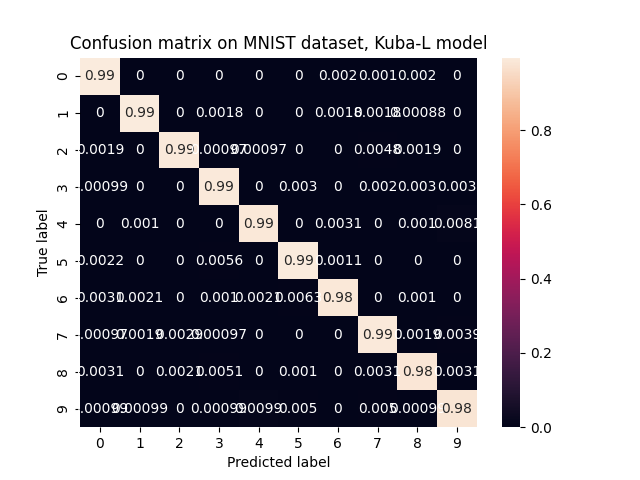
\includegraphics[width=\linewidth]{img/kuba/mnist/large_cm.png}
        \caption{Macierz pomyłek}
    \end{subfigure}
    \caption{Wyniki dla 1 architektury (Train acc: 0.997; Test acc: 0.987)}
\end{figure}


\subsection*{Druga architektura, prowadząca do ekstrakcji 2 cech}


\pgfplotstableread[col sep=comma]{data/kuba/mnist/smol.csv}\kubaMnistSmol{}

\begin{figure}[H]\centering
    \begin{subfigure}[t]{.55\textwidth}
        \plotAccuraciesFromLoggedMetrics{\kubaMnistSmol}
        \caption{Wykres zmian accuracy}
    \end{subfigure}
    \hspace{2em}
    \begin{subfigure}[t]{.34\textwidth}
        \centering
        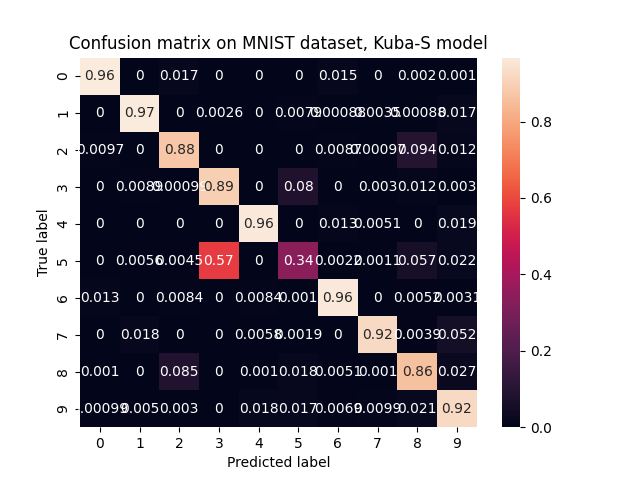
\includegraphics[width=\linewidth]{img/kuba/mnist/smol_cm.png}
        \caption{Macierz pomyłek}
    \end{subfigure}
    \caption{Wyniki dla 2 architektury (Train acc: 0.836;Test acc: 0.566)}\label{fig:kuba/mnist/smol}
\end{figure}

\begin{wrapfigure}[5]{r}{0.25\textwidth}
    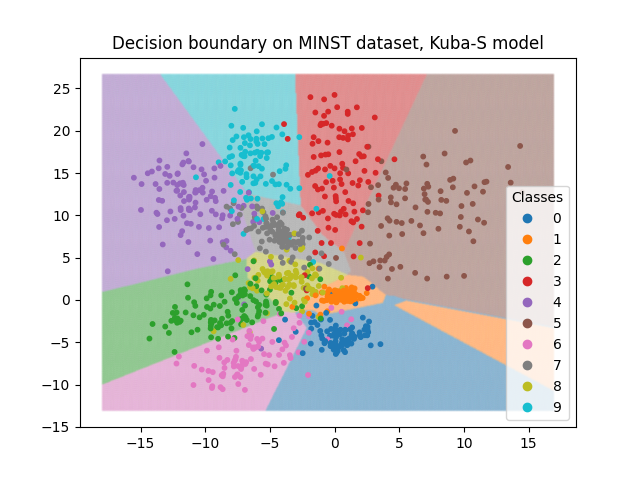
\includegraphics[width=\linewidth]{img/kuba/mnist/smol_db.png}
    \caption{Granica decyzyjna dla arch.~2}\label{fig:kuba/mnist/smol/decision_boundary}
\end{wrapfigure}

W drugiej architekturze warunkiem koniecznym jest rozmiar wektora cech, wynoszący 2 cechy.
Jest to umotywowane chęcią stworzenia wizualizacji granic decyzyjnych.
Ekstraktor cech składa się z następujących warstw:
\tiny
\begin{verbatim}
(feature_extractor): Sequential(
    (0): Conv2d(1, 10, kernel_size=(5, 5), stride=(1, 1), padding=(2, 2))
    (1): ReLU()
    (2): Dropout2d(p=0.1, inplace=False)
    (3): MaxPool2d(kernel_size=2, stride=2, padding=0, dilation=1, ceil_mode=False)
    (4): Conv2d(10, 5, kernel_size=(5, 5), stride=(1, 1))
    (5): ReLU()
    (6): MaxPool2d(kernel_size=2, stride=2, padding=0, dilation=1, ceil_mode=False)
    (7): Conv2d(5, 2, kernel_size=(3, 3), stride=(1, 1))
    (8): ReLU()
    (9): Flatten(start_dim=1, end_dim=-1)
    (10): Linear(in_features=18, out_features=2, bias=True)
)
(classifier): Sequential(
    (0): Linear(in_features=2, out_features=5, bias=True)
    (1): ReLU()
    (2): Linear(in_features=5, out_features=10, bias=True)
)
\end{verbatim}
\normalsize

W tym modelu, aby jeszcze bardziej zmniejszyć ilość cech, zastosowano jeszcze jedną warstwę konwolucyjną.
Finalnie, ekstraktor cech zawiera jedną w pełni połączoną warstwę, w celu redukcji do 2 cech.

W tym modelu postanowiono również przeprowadzić eksperyment z użyciem warstwy dropout w celu poprawienia
odporności na overfitting.
Pomimo, że z racji na dużą liczność zbioru treningowego, w eksperymencie 1 nie ma dużego ryzyka przetrenowania, 
sytuacja może ulec zmianie w eksperymencie 2. Negatywnym efektem użycia warstwy dropout jest spowolnienie procesu uczenia, co jest dobrze widoczne na wykresie.

Warstwy konwolucyjne prowadzą do finalnego tensora o wymiarach $2 \times 3 \times 3$, 10więc na końcu ekstraktora cech znajduje się jeszce jenda warstwa linear, tworząca 2-wymiarowy wektor cech.

Klasyfikator zawiera jedną warstwę ukrytą o rozmiarze 5 neuronów, z funkcją relu, a następnie warstwę wyjściową o rozmiarze 10 neuronów.

\pagebreak
\section{Eksperyment 1: Architektury sieci splotowej dla MNIST (Magdalena Pakuła)}\label{sec:ex1-pakula_mnist}

\subsection*{Pierwsza architektura}
Zawiera trzy warstwy splotowe każda warstwa wydobywa coraz bardziej abstrakcyjne cechy. Warstwy początkowe rejestrują krawędzie i tekstury, podczas gdy warstwy głębsze rejestrują kształty i bardziej złożone wzory. Ma to kluczowe znaczenie w przypadku rozpoznawania cyfr, gdzie należy rozróżnić subtelne różnice.
Po każdej wartwie splotowej następuje redukcja wymiarowości, dzięki użyciu MaxPool2d, co pozwala sieci skupić się na najbardziej istotnych cechach cyfr, poprawiając generalizację.
Stopniowy wzrost filtrów (zaczynając od 8, a kończąc na 32) zapewnia równowagę między wydajnością obliczeniową a bogactwem funkcji.
Ostatecznie model zostaje spłaszczony do 288 obiektów, wystarczającą pojemność do reprezentowania złożonych wzorów, nie będąc jednocześnie zbyt dużym, co mogłoby prowadzić do nadmiernego dopasowania.
Rezultaty tej metody zostały przedstawione poniżej na wykresie accuracy, macierzy pomyłek i wyników accurracy i loss najlepszego modelu na rys. ~\ref{fig:exp1_magda_mnist}.

\pgfplotstableread[col sep=comma]{data/magda/mnist/large.csv}\MagdaMnistLarge{}

\begin{figure}[H]\centering
    \begin{subfigure}[b]{.4\textwidth}
        \plotAccuraciesFromLoggedMetrics{\MagdaMnistLarge}
        \caption{Wykres zmian accuracy}
    \end{subfigure}
    \begin{subfigure}[b]{.24\textwidth}
        \centering
        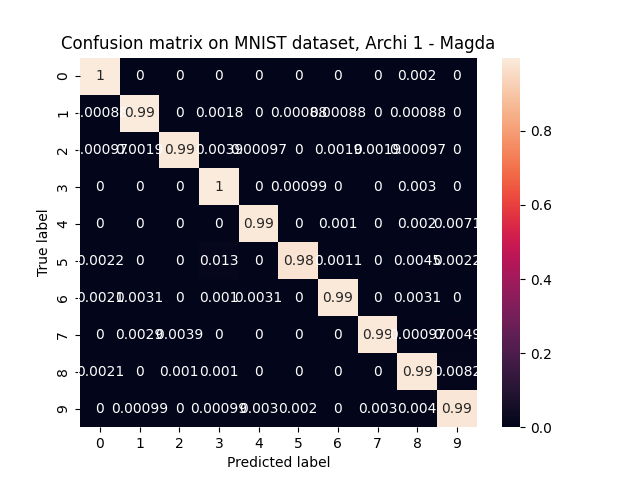
\includegraphics[width=\linewidth]{img/magda/MNIST_large_matrix}
        \caption{Macierz pomyłek}
    \end{subfigure}
    \begin{subfigure}[b]{.24\textwidth}
        \centering
        \scriptsize
        \begin{tabular}{|c|c|}
            \hline
            Test metric & Result \\
            \hline
            Test acc & 0.984 \\
            Test loss & 0.045 \\
            \hline
        \end{tabular}
        \caption{Wyniki accuracy i loss najlepszego modelu (epoch 5)}
    \end{subfigure}
    \caption{Wyniki dla 1 architektury}
    \label{fig:exp1_magda_mnist}
\end{figure}


\subsection*{Druga architektura, prowadząca do ekstrakcji 2 cech}
Składa się z czterech warstw splotowych. Liczba filtrów w tych warstwach jest hierarchicznie zwiększana od 32 do 128. Po każdej warstwie splotowej następuje normalizacja wsadowa (BatchNorm2d), funkcja aktywacji ReLU i redukcja wymiarowości poprzez użycie operacji MaxPool2d, z wyjątkiem ostatniej warstwy, gdzie ta operacja nie jest już potrzebna.
Taka konfiguracja została zaprojektowana w celu stopniowego wyodrębniania coraz bardziej skomplikowanych cech z obrazów MNIST. Pierwsze warstwy koncentrują się na wykrywaniu podstawowych cech, takich jak krawędzie i rogi, dzięki mniejszej liczbie filtrów. Następnie, w kolejnych warstwach, liczba filtrów jest stopniowo zwiększana.
Operacje normalizacji wsadowej pomagają w stabilizacji uczenia poprzez zapewnienie jednolitego zakresu wartości na wyjściu z każdej warstwy, co może przyspieszyć proces uczenia oraz poprawić ogólną wydajność sieci. Funkcja aktywacji ReLU została wybrana z powodu jej skuteczności w eliminowaniu zjawiska zanikającego gradientu i aktywowania jedynie istotnych cech.

Rezultaty tej metody zostały przedstawione poniżej na rys. ~\ref{fig:exp1_magda_mnist2}.

\pgfplotstableread[col sep=comma]{data/magda/mnist/small.csv}\MagdaMnistSmall{}

\begin{figure}[H]\centering
    \begin{subfigure}[b]{.4\textwidth}
        \plotAccuraciesFromLoggedMetrics{\MagdaMnistSmall}
        \caption{Wykres zmian accuracy}
    \end{subfigure}
    \begin{subfigure}[b]{.19\textwidth}
        \centering
        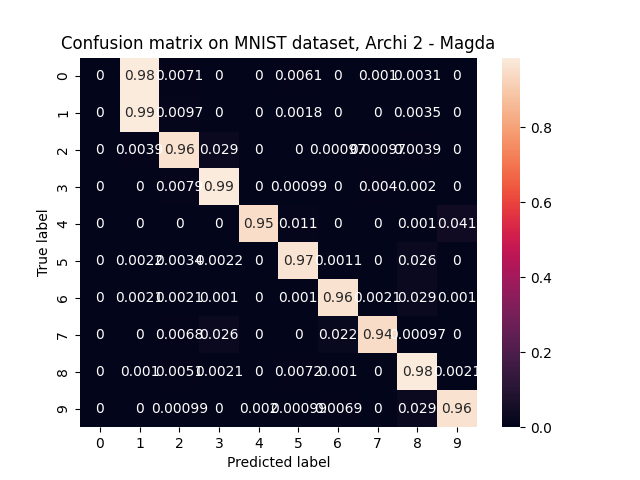
\includegraphics[width=\linewidth]{img/magda/MNIST_small_matrix}
        \caption{Macierz pomyłek}
    \end{subfigure}
    \begin{subfigure}[b]{.19\textwidth}
        \centering
        \scriptsize
        \begin{tabular}{|c|c|}
            \hline
            Test metric & Result \\
            \hline
            Test acc & 0.869 \\
            Test loss & 0.388 \\
            \hline
        \end{tabular}
        \caption{Wyniki accuracy i loss najlepszego modelu (epoch 5)}
    \end{subfigure}
    \begin{subfigure}[b]{.19\textwidth}
        \centering
        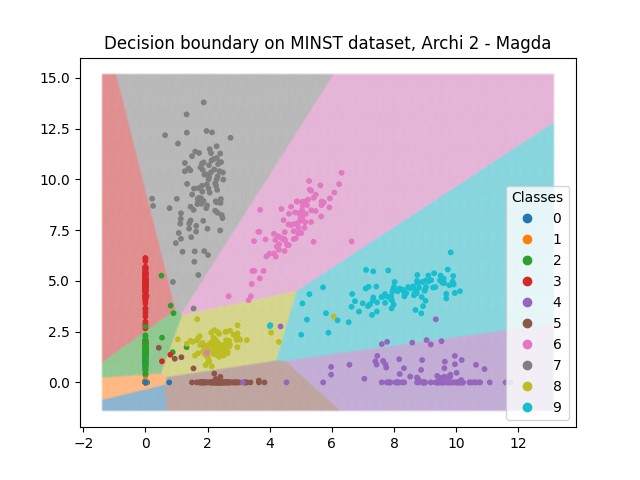
\includegraphics[width=\linewidth]{img/magda/MNIST_small_decision}
        \caption{Wizualizacja granic decyzyjnych}
    \end{subfigure}
    \caption{Wyniki dla 2 architektury}\label{fig:exp1_magda_mnist2}
\end{figure}

\pagebreak
\section{Eksperyment 1: Architektury sieci splotowej dla CIFAR10 (Jakub Pawlak)}\label{sec:ex1-pawlak_cifar}

\subsection*{Pierwsza architektura}

\pgfplotstableread[col sep=comma]{data/kuba/cifar/large.csv}\kubaCifarLarge{}

\tiny
\begin{verbatim}
(feature_extractor): _CIFARLargeFeatureExtractor(
    (step_1): Sequential(
        (0): Conv2d(3, 64, kernel_size=(3, 3), stride=(1, 1), padding=(1, 1))
        (1): BatchNorm2d(64, eps=1e-05, momentum=0.1, affine=True, track_running_stats=True)
        (2): ReLU()
        (3): Conv2d(64, 128, kernel_size=(3, 3), stride=(1, 1), padding=(1, 1))
        (4): BatchNorm2d(128, eps=1e-05, momentum=0.1, affine=True, track_running_stats=True)
        (5): ReLU()
        (6): MaxPool2d(kernel_size=2, stride=2, padding=0, dilation=1, ceil_mode=False)
    )
    (residual_1): Sequential(
        (0): Conv2d(128, 128, kernel_size=(3, 3), stride=(1, 1), padding=(1, 1))
        (1): BatchNorm2d(128, eps=1e-05, momentum=0.1, affine=True, track_running_stats=True)
        (2): ReLU()
        (3): Conv2d(128, 128, kernel_size=(3, 3), stride=(1, 1), padding=(1, 1))
        (4): BatchNorm2d(128, eps=1e-05, momentum=0.1, affine=True, track_running_stats=True)
        (5): ReLU()
    )
    (step_2): Sequential(
        (0): Conv2d(128, 64, kernel_size=(3, 3), stride=(1, 1), padding=(1, 1))
        (1): BatchNorm2d(64, eps=1e-05, momentum=0.1, affine=True, track_running_stats=True)
        (2): ReLU()
        (3): MaxPool2d(kernel_size=2, stride=2, padding=0, dilation=1, ceil_mode=False)
    )
    (residual_2): Sequential(
        (0): Conv2d(64, 64, kernel_size=(3, 3), stride=(1, 1), padding=(1, 1))
        (1): BatchNorm2d(64, eps=1e-05, momentum=0.1, affine=True, track_running_stats=True)
        (2): ReLU()
        (3): Conv2d(64, 64, kernel_size=(3, 3), stride=(1, 1), padding=(1, 1))
        (4): BatchNorm2d(64, eps=1e-05, momentum=0.1, affine=True, track_running_stats=True)
        (5): ReLU()
    )
    (step_3): Sequential(
        (0): Conv2d(64, 16, kernel_size=(3, 3), stride=(1, 1), padding=(1, 1))
        (1): BatchNorm2d(16, eps=1e-05, momentum=0.1, affine=True, track_running_stats=True)
        (2): ReLU()
        (3): MaxPool2d(kernel_size=2, stride=2, padding=0, dilation=1, ceil_mode=False)
    )
)
(classifier): Sequential(
    (0): Linear(in_features=256, out_features=64, bias=True)
    (1): ReLU()
    (2): Linear(in_features=64, out_features=16, bias=True)
    (3): ReLU()
    (4): Linear(in_features=16, out_features=10, bias=True)
)
\end{verbatim}
\normalsize


\begin{figure}[H]\centering
    \begin{subfigure}[t]{.55\textwidth}
        \plotAccuraciesFromLoggedMetrics{\kubaCifarLarge}
        \caption{Wykres zmian accuracy}
    \end{subfigure}
    \hspace{2em}
    \begin{subfigure}[t]{.34\textwidth}
        \centering
        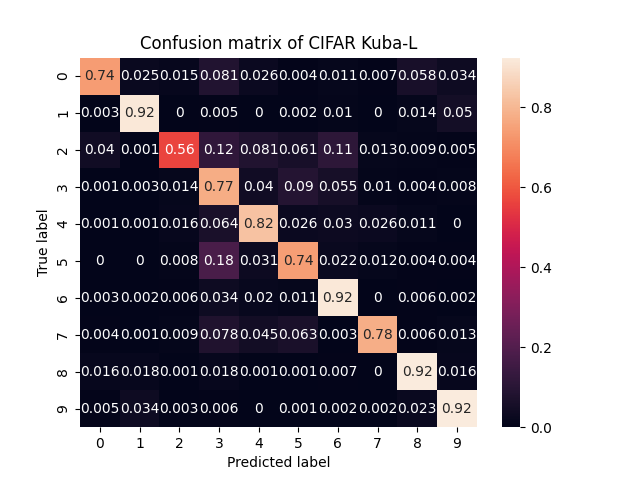
\includegraphics[width=\linewidth]{img/kuba/cifar/large_cm.png}
        \caption{Macierz pomyłek}
    \end{subfigure}
    \caption{Wyniki dla 1 architektury (Train acc: 0.931; Test acc: 0.810)}
\end{figure}


\subsection*{Druga architektura prowadząca do ekstrakcji 2 cech}

\pgfplotstableread[col sep=comma]{data/kuba/cifar/smol.csv}\kubaCifarSmol{}

\begin{figure}[H]\centering
    \begin{subfigure}[t]{.55\textwidth}
        \plotAccuraciesFromLoggedMetrics{\kubaCifarSmol}
        \caption{Wykres zmian accuracy}
    \end{subfigure}
    \hspace{2em}
    \begin{subfigure}[t]{.34\textwidth}
        \centering
        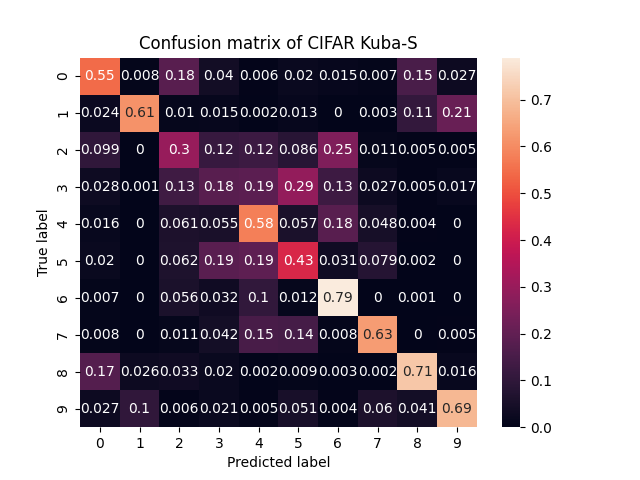
\includegraphics[width=\linewidth]{img/kuba/cifar/smol_cm.png}
        \caption{Macierz pomyłek}
    \end{subfigure}
    \caption{Wyniki dla 2 architektury (Train acc: 0.607; Test acc: 0.547)}
\end{figure}

\small
\begin{verbatim}
(feature_extractor): Sequential(
    (0): Conv2d(3, 64, kernel_size=(3, 3), stride=(1, 1), padding=(1, 1))
    (1): BatchNorm2d(64, eps=1e-05, momentum=0.1, affine=True, track_running_stats=True)
    (2): ReLU()
    (3): MaxPool2d(kernel_size=2, stride=2, padding=0, dilation=1, ceil_mode=False)
    (4): Conv2d(64, 32, kernel_size=(3, 3), stride=(1, 1), padding=(1, 1))
    (5): BatchNorm2d(32, eps=1e-05, momentum=0.1, affine=True, track_running_stats=True)
    (6): ReLU()
    (7): MaxPool2d(kernel_size=2, stride=2, padding=0, dilation=1, ceil_mode=False)
    (8): Conv2d(32, 8, kernel_size=(3, 3), stride=(1, 1), padding=(1, 1))
    (9): ReLU()
    (10): MaxPool2d(kernel_size=2, stride=2, padding=0, dilation=1, ceil_mode=False)
    (11): Conv2d(8, 2, kernel_size=(4, 4), stride=(1, 1))
    (12): Flatten(start_dim=1, end_dim=-1)
)
(classifier): Sequential(
    (0): Linear(in_features=2, out_features=16, bias=True)
    (1): ReLU()
    (2): Linear(in_features=16, out_features=10, bias=True)
)
\end{verbatim}
\normalsize

\pagebreak
\section{Eksperyment 1: Architektury sieci splotowej dla CIFAR10 (Magdalena Pakuła)}\label{sec:ex1-pakula_cifar}

\subsection*{Pierwsza architektura}
Składa się z trzech warstw splotowych, gdzie każda z nich wykorzystuje coraz większą liczbę filtrów o rozmiarze 3x3
Pierwsza warstwa splotowa zawiera 32 filtry, stosuje funkcję aktywacji ReLU oraz warstwę Dropout z współczynnikiem 0.2, która losowo wyłącza część neuronów, zapobiegając nadmiernemu dopasowaniu. Następnie warstwa MaxPooling zmniejsza rozmiar przestrzenny danych o połowę. Druga warstwa splotowa składa się z 64 filtrów, ponownie stosuje ReLU oraz Dropout z współczynnikiem 0.3, a także warstwę MaxPooling, która zmniejsza rozmiar przestrzenny danych do 8x8. Trzecia warstwa splotowa zawiera 128 filtrów, stosuje ReLU, Dropout z współczynnikiem 0.4 oraz MaxPooling, zmniejszając rozmiar przestrzenny danych do 4x4. Dane są następnie spłaszczone do jednowymiarowego tensora za pomocą warstwy Flatten, umożliwiając przekazanie ich do warstw w pełni połączonych w celu klasyfikacji. Klasyfikator składa się z dwóch warstw w pełni połączonych, gdzie pierwsza redukuje rozmiar cech do 128, stosując funkcję ReLU oraz Dropout z współczynnikiem 0.5, a druga warstwa klasyfikuje dane do liczby klas
Ta architektura została zoptymalizowana w celu efektywnego wyodrębniania cech z obrazów o niskiej rozdzielczości, takich jak te występujące w zbiorze CIFAR. Większa liczba warstw splotowych oraz zwiększenie liczby filtrów w każdej warstwie pozwalają na lepsze modelowanie danych
Rezultaty tej metody zostały przedstawione na rys. ~\ref{fig:exp1_magda_cifar}.

\pgfplotstableread[col sep=comma]{data/magda/cifar/large.csv}\MagdaCifarLarge{}

\begin{figure}[H]\centering
    \begin{subfigure}[b]{.4\textwidth}
        \plotAccuraciesFromLoggedMetrics{\MagdaCifarLarge}
        \caption{Wykres zmian accuracy}
    \end{subfigure}
    \begin{subfigure}[b]{.24\textwidth}
        \centering
        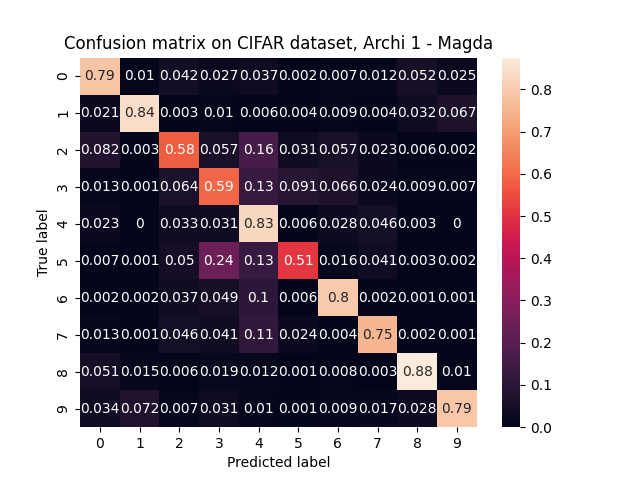
\includegraphics[width=\linewidth]{img/magda/CIFAR_large_matrix}
        \caption{Macierz pomyłek}
    \end{subfigure}
    \begin{subfigure}[b]{.24\textwidth}
        \centering
        \scriptsize
        \begin{tabular}{|c|c|}
            \hline
            Test metric & Result \\
            \hline
            Test accuracy & 0.735 \\
            Test loss & 0.841 \\
            \hline
        \end{tabular}
        \caption{Wyniki accuracy i loss najlepszego modelu (epoch 7)}
    \end{subfigure}
    \caption{Wyniki dla 1 architektury}
    \label{fig:exp1_magda_cifar}
\end{figure}


\subsection*{Druga architektura prowadząca do ekstrakcji 2 cech}
Składa się z 4 warstw splotowych z 32, 64 i 128 filtrami, które pozwalają na stopniowe wyodrębnianie coraz bardziej złożonych
cech z danych wejściowych. Następie użycie BatchNorm2d stabilizuje proces treningu i pozwala na szybsze uczenie się modelu,
a funkcja aktywacji ReLU wprowadza nieliniowość. Następnie jest wartswa MaxPooling redukująca rozmiar danych.
Ostatnia warstwa splotowa prowadzi do 2 filtrów. A na końcu dodana jest Ffnkcja aktywacji ReLU.
Klasyfikator składa się z trzech warstw w pełni połączonych, które stopniowo redukują rozmiar cech i umożliwiają klasyfikację danych do odpowiedniej liczby klas. Dropout (0.3) w pierwszej warstwie w pełni połączonej zapobiega nadmiernemu dopasowaniu modelu poprzez losowe wyłączanie neuronów podczas treningu.

Rezultaty przedstawione są na rys. ~\ref{fig:exp1_magda_cifar2}.

\pgfplotstableread[col sep=comma]{data/magda/cifar/small.csv}\MagdaCifarSmall{}

\begin{figure}[H]\centering
    \begin{subfigure}[b]{.4\textwidth}
        \plotAccuraciesFromLoggedMetrics{\MagdaCifarSmall}
        \caption{Wykres zmian accuracy}
    \end{subfigure}
    \begin{subfigure}[b]{.19\textwidth}
        \centering
        \includegraphics[width=\linewidth]{img/magda/Cifar_small_matrix}
        \caption{Macierz pomyłek}
    \end{subfigure}
    \begin{subfigure}[b]{.19\textwidth}
        \centering
        \scriptsize
        \begin{tabular}{|c|c|}
            \hline
            Test metric & Result \\
            \hline
            Test acc & 0.573 \\
            Test loss & 1.216 \\
            \hline
        \end{tabular}
        \caption{Wyniki accuracy i loss najlepszego modelu (epoch 10)}
    \end{subfigure}
    \begin{subfigure}[b]{.19\textwidth}
        \centering
        \includegraphics[width=\linewidth]{img/magda/Cifar_small_decision}
        \caption{Wizualizacja granic decyzyjnych}
    \end{subfigure}
    \caption{Wyniki dla 2 architektury}
    \label{fig:exp1_magda_cifar2}
\end{figure}

\pagebreak
\section{Eksperyment 2: Wyniki dla MNIST}\label{sec:ex2_mnist}

\paragraph{Najlepsza architektura}
\paragraph{Najelpsza architektura prowadząca do ekstrakcji 2 cech}

\pagebreak
\section{Eksperyment 2: Wyniki dla CIFAR10}\label{sec:ex2_cifar}

\paragraph{Najlepsza architektura}
\paragraph{Najelpsza architektura prowadząca do ekstrakcji 2 cech}

\pagebreak
\section{Analiza i wnioski}\label{sec:wyniki}
\subsection*{Porównanie architektur sieci splotowych}
Generalne wnioski Magdy dla MNIST\@: wyszlo zajebiscie, rezultaty same pokazuja --- mozna sie bić :)
Generalne wnioski Magdy dla CIFAR\@: nie wyszlo zajebiscie, wyniki sa słabe. Dla 1 archi nie udalo mi sie stworzyc modelu ktory by nie robil underfittug --- wszystkie mniej czy wiecej to robily, a dla zachowania podobnych experymentow co Kuba to nie zmienialam learning rate. Zmienialam relu, conv layers, filters ale obecny model to moj najlepszy.
Jesli chodzi o Archi 2 to tez moj najlepszy model ktory stworzylam, mamy znowu lekki underfitting
wiadomka ze dla 2 cech beda to znacznie gorsze wyniki w szczegolnosci dla tak skomplikownych i nieczytelnych obrazkow jak CIFAR.
--
Model Kuby dla Cifara jest better bo\ldots --- tutaj wyjasnienie czemu jest taki boski.
\subsection*{Wpływ augmentacji danych}

\end{document}